\documentclass[1p]{elsarticle_modified}
%\bibliographystyle{elsarticle-num}

%\usepackage[colorlinks]{hyperref}
%\usepackage{abbrmath_seonhwa} %\Abb, \Ascr, \Acal ,\Abf, \Afrak
\usepackage{amsfonts}
\usepackage{amssymb}
\usepackage{amsmath}
\usepackage{amsthm}
\usepackage{scalefnt}
\usepackage{amsbsy}
\usepackage{kotex}
\usepackage{caption}
\usepackage{subfig}
\usepackage{color}
\usepackage{graphicx}
\usepackage{xcolor} %% white, black, red, green, blue, cyan, magenta, yellow
\usepackage{float}
\usepackage{setspace}
\usepackage{hyperref}

\usepackage{tikz}
\usetikzlibrary{arrows}

\usepackage{multirow}
\usepackage{array} % fixed length table
\usepackage{hhline}

%%%%%%%%%%%%%%%%%%%%%
\makeatletter
\renewcommand*\env@matrix[1][\arraystretch]{%
	\edef\arraystretch{#1}%
	\hskip -\arraycolsep
	\let\@ifnextchar\new@ifnextchar
	\array{*\c@MaxMatrixCols c}}
\makeatother %https://tex.stackexchange.com/questions/14071/how-can-i-increase-the-line-spacing-in-a-matrix
%%%%%%%%%%%%%%%

\usepackage[normalem]{ulem}

\newcommand{\msout}[1]{\ifmmode\text{\sout{\ensuremath{#1}}}\else\sout{#1}\fi}
%SOURCE: \msout is \stkout macro in https://tex.stackexchange.com/questions/20609/strikeout-in-math-mode

\newcommand{\cancel}[1]{
	\ifmmode
	{\color{red}\msout{#1}}
	\else
	{\color{red}\sout{#1}}
	\fi
}

\newcommand{\add}[1]{
	{\color{blue}\uwave{#1}}
}

\newcommand{\replace}[2]{
	\ifmmode
	{\color{red}\msout{#1}}{\color{blue}\uwave{#2}}
	\else
	{\color{red}\sout{#1}}{\color{blue}\uwave{#2}}
	\fi
}

\newcommand{\Sol}{\mathcal{S}} %segment
\newcommand{\D}{D} %diagram
\newcommand{\A}{\mathcal{A}} %arc


%%%%%%%%%%%%%%%%%%%%%%%%%%%%%5 test

\def\sl{\operatorname{\textup{SL}}(2,\Cbb)}
\def\psl{\operatorname{\textup{PSL}}(2,\Cbb)}
\def\quan{\mkern 1mu \triangleright \mkern 1mu}

\theoremstyle{definition}
\newtheorem{thm}{Theorem}[section]
\newtheorem{prop}[thm]{Proposition}
\newtheorem{lem}[thm]{Lemma}
\newtheorem{ques}[thm]{Question}
\newtheorem{cor}[thm]{Corollary}
\newtheorem{defn}[thm]{Definition}
\newtheorem{exam}[thm]{Example}
\newtheorem{rmk}[thm]{Remark}
\newtheorem{alg}[thm]{Algorithm}

\newcommand{\I}{\sqrt{-1}}
\begin{document}

%\begin{frontmatter}
%
%\title{Boundary parabolic representations of knots up to 8 crossings}
%
%%% Group authors per affiliation:
%\author{Yunhi Cho} 
%\address{Department of Mathematics, University of Seoul, Seoul, Korea}
%\ead{yhcho@uos.ac.kr}
%
%
%\author{Seonhwa Kim} %\fnref{s_kim}}
%\address{Center for Geometry and Physics, Institute for Basic Science, Pohang, 37673, Korea}
%\ead{ryeona17@ibs.re.kr}
%
%\author{Hyuk Kim}
%\address{Department of Mathematical Sciences, Seoul National University, Seoul 08826, Korea}
%\ead{hyukkim@snu.ac.kr}
%
%\author{Seokbeom Yoon}
%\address{Department of Mathematical Sciences, Seoul National University, Seoul, 08826,  Korea}
%\ead{sbyoon15@snu.ac.kr}
%
%\begin{abstract}
%We find all boundary parabolic representation of knots up to 8 crossings.
%
%\end{abstract}
%\begin{keyword}
%    \MSC[2010] 57M25 
%\end{keyword}
%
%\end{frontmatter}

%\linenumbers
%\tableofcontents
%
\newcommand\colored[1]{\textcolor{white}{\rule[-0.35ex]{0.8em}{1.4ex}}\kern-0.8em\color{red} #1}%
%\newcommand\colored[1]{\textcolor{white}{ #1}\kern-2.17ex	\textcolor{white}{ #1}\kern-1.81ex	\textcolor{white}{ #1}\kern-2.15ex\color{red}#1	}

{\Large $\underline{12a_{0781}~(K12a_{0781})}$}

\setlength{\tabcolsep}{10pt}
\renewcommand{\arraystretch}{1.6}
\vspace{1cm}\begin{tabular}{m{100pt}>{\centering\arraybackslash}m{274pt}}
\multirow{5}{120pt}{
	\centering
	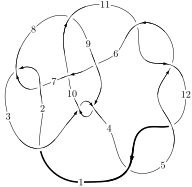
\includegraphics[width=112pt]{../../../GIT/diagram.site/Diagrams/png/1582_12a_0781.png}\\
\ \ \ A knot diagram\footnotemark}&
\allowdisplaybreaks
\textbf{Linearized knot diagam} \\
\cline{2-2}
 &
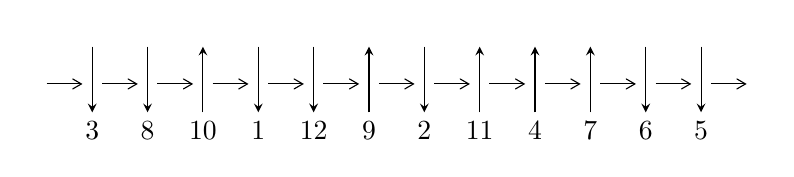
\begin{tikzpicture}[x=20pt, y=17pt]
	% nodes
	\node (C0) at (0, 0) {};
	\node (C1) at (1, 0) {};
	\node (C1U) at (1, +1) {};
	\node (C1D) at (1, -1) {3};

	\node (C2) at (2, 0) {};
	\node (C2U) at (2, +1) {};
	\node (C2D) at (2, -1) {8};

	\node (C3) at (3, 0) {};
	\node (C3U) at (3, +1) {};
	\node (C3D) at (3, -1) {10};

	\node (C4) at (4, 0) {};
	\node (C4U) at (4, +1) {};
	\node (C4D) at (4, -1) {1};

	\node (C5) at (5, 0) {};
	\node (C5U) at (5, +1) {};
	\node (C5D) at (5, -1) {12};

	\node (C6) at (6, 0) {};
	\node (C6U) at (6, +1) {};
	\node (C6D) at (6, -1) {9};

	\node (C7) at (7, 0) {};
	\node (C7U) at (7, +1) {};
	\node (C7D) at (7, -1) {2};

	\node (C8) at (8, 0) {};
	\node (C8U) at (8, +1) {};
	\node (C8D) at (8, -1) {11};

	\node (C9) at (9, 0) {};
	\node (C9U) at (9, +1) {};
	\node (C9D) at (9, -1) {4};

	\node (C10) at (10, 0) {};
	\node (C10U) at (10, +1) {};
	\node (C10D) at (10, -1) {7};

	\node (C11) at (11, 0) {};
	\node (C11U) at (11, +1) {};
	\node (C11D) at (11, -1) {6};

	\node (C12) at (12, 0) {};
	\node (C12U) at (12, +1) {};
	\node (C12D) at (12, -1) {5};
	\node (C13) at (13, 0) {};

	% arrows
	\draw[->,>={angle 60}]
	(C0) edge (C1) (C1) edge (C2) (C2) edge (C3) (C3) edge (C4) (C4) edge (C5) (C5) edge (C6) (C6) edge (C7) (C7) edge (C8) (C8) edge (C9) (C9) edge (C10) (C10) edge (C11) (C11) edge (C12) (C12) edge (C13) ;	\draw[->,>=stealth]
	(C1U) edge (C1D) (C2U) edge (C2D) (C3D) edge (C3U) (C4U) edge (C4D) (C5U) edge (C5D) (C6D) edge (C6U) (C7U) edge (C7D) (C8D) edge (C8U) (C9D) edge (C9U) (C10D) edge (C10U) (C11U) edge (C11D) (C12U) edge (C12D) ;
	\end{tikzpicture} \\
\hhline{~~} \\& 
\textbf{Solving Sequence} \\ \cline{2-2} 
 &
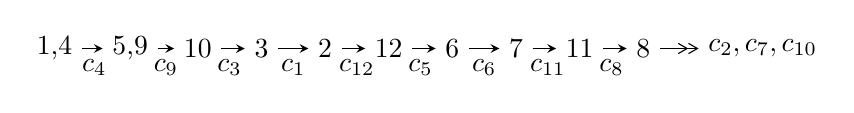
\begin{tikzpicture}[x=23pt, y=7pt]
	% node
	\node (A0) at (-1/8, 0) {1,4};
	\node (A1) at (17/16, 0) {5,9};
	\node (A2) at (17/8, 0) {10};
	\node (A3) at (25/8, 0) {3};
	\node (A4) at (33/8, 0) {2};
	\node (A5) at (41/8, 0) {12};
	\node (A6) at (49/8, 0) {6};
	\node (A7) at (57/8, 0) {7};
	\node (A8) at (65/8, 0) {11};
	\node (A9) at (73/8, 0) {8};
	\node (C1) at (1/2, -1) {$c_{4}$};
	\node (C2) at (13/8, -1) {$c_{9}$};
	\node (C3) at (21/8, -1) {$c_{3}$};
	\node (C4) at (29/8, -1) {$c_{1}$};
	\node (C5) at (37/8, -1) {$c_{12}$};
	\node (C6) at (45/8, -1) {$c_{5}$};
	\node (C7) at (53/8, -1) {$c_{6}$};
	\node (C8) at (61/8, -1) {$c_{11}$};
	\node (C9) at (69/8, -1) {$c_{8}$};
	\node (A10) at (11, 0) {$c_{2},c_{7},c_{10}$};

	% edge
	\draw[->,>=stealth]	
	(A0) edge (A1) (A1) edge (A2) (A2) edge (A3) (A3) edge (A4) (A4) edge (A5) (A5) edge (A6) (A6) edge (A7) (A7) edge (A8) (A8) edge (A9) ;
	\draw[->>,>={angle 60}]	
	(A9) edge (A10);
\end{tikzpicture} \\ 

\end{tabular} \\

\footnotetext{
The image of knot diagram is generated by the software ``\textbf{Draw programme}" developed by Andrew Bartholomew(\url{http://www.layer8.co.uk/maths/draw/index.htm\#Running-draw}), where we modified some parts for our purpose(\url{https://github.com/CATsTAILs/LinksPainter}).
}\phantom \\ \newline 
\centering \textbf{Ideals for irreducible components\footnotemark of $X_{\text{par}}$} 
 
\begin{align*}
I^u_{1}&=\langle 
-3.86638\times10^{158} u^{97}-6.01764\times10^{158} u^{96}+\cdots+2.14603\times10^{159} b+2.00594\times10^{160},\\
\phantom{I^u_{1}}&\phantom{= \langle  }-5.79119\times10^{159} u^{97}-1.25565\times10^{160} u^{96}+\cdots+4.07746\times10^{160} a-2.67995\times10^{161},\\
\phantom{I^u_{1}}&\phantom{= \langle  }u^{98}+2 u^{97}+\cdots+145 u+19\rangle \\
I^u_{2}&=\langle 
- u^{17}- u^{16}+\cdots+b-7 u,\;u^{19}+u^{18}+\cdots+a-2,\;u^{20}+u^{19}+\cdots+14 u^2+1\rangle \\
\\
\end{align*}
\raggedright * 2 irreducible components of $\dim_{\mathbb{C}}=0$, with total 118 representations.\\
\footnotetext{All coefficients of polynomials are rational numbers. But the coefficients are sometimes approximated in decimal forms when there is not enough margin.}
\newpage
\renewcommand{\arraystretch}{1}
\centering \section*{I. $I^u_{1}= \langle -3.87\times10^{158} u^{97}-6.02\times10^{158} u^{96}+\cdots+2.15\times10^{159} b+2.01\times10^{160},\;-5.79\times10^{159} u^{97}-1.26\times10^{160} u^{96}+\cdots+4.08\times10^{160} a-2.68\times10^{161},\;u^{98}+2 u^{97}+\cdots+145 u+19 \rangle$}
\flushleft \textbf{(i) Arc colorings}\\
\begin{tabular}{m{7pt} m{180pt} m{7pt} m{180pt} }
\flushright $a_{1}=$&$\begin{pmatrix}0\\u\end{pmatrix}$ \\
\flushright $a_{4}=$&$\begin{pmatrix}1\\0\end{pmatrix}$ \\
\flushright $a_{5}=$&$\begin{pmatrix}1\\u^2\end{pmatrix}$ \\
\flushright $a_{9}=$&$\begin{pmatrix}0.142029 u^{97}+0.307949 u^{96}+\cdots+14.8737 u+6.57260\\0.180164 u^{97}+0.280408 u^{96}+\cdots-42.6979 u-9.34719\end{pmatrix}$ \\
\flushright $a_{10}=$&$\begin{pmatrix}0.322194 u^{97}+0.588357 u^{96}+\cdots-27.8242 u-2.77458\\0.180164 u^{97}+0.280408 u^{96}+\cdots-42.6979 u-9.34719\end{pmatrix}$ \\
\flushright $a_{3}=$&$\begin{pmatrix}-0.381407 u^{97}-1.32617 u^{96}+\cdots-330.089 u-43.7156\\-0.612689 u^{97}-1.81913 u^{96}+\cdots-217.338 u-25.7105\end{pmatrix}$ \\
\flushright $a_{2}=$&$\begin{pmatrix}0.949339 u^{97}+2.86582 u^{96}+\cdots+583.792 u+72.2286\\-0.741603 u^{97}-1.00302 u^{96}+\cdots+129.459 u+23.7288\end{pmatrix}$ \\
\flushright $a_{12}=$&$\begin{pmatrix}u\\u^3+u\end{pmatrix}$ \\
\flushright $a_{6}=$&$\begin{pmatrix}u^2+1\\u^4+2 u^2\end{pmatrix}$ \\
\flushright $a_{7}=$&$\begin{pmatrix}0.695299 u^{97}+1.05722 u^{96}+\cdots+35.9036 u-7.81290\\0.504732 u^{97}+1.15514 u^{96}+\cdots+214.872 u+27.8479\end{pmatrix}$ \\
\flushright $a_{11}=$&$\begin{pmatrix}u^3+2 u\\u^5+3 u^3+u\end{pmatrix}$ \\
\flushright $a_{8}=$&$\begin{pmatrix}0.299319 u^{97}+0.487641 u^{96}+\cdots-41.9938 u-4.74001\\0.221229 u^{97}+0.313332 u^{96}+\cdots-46.7994 u-11.0038\end{pmatrix}$\\&\end{tabular}
\flushleft \textbf{(ii) Obstruction class $= -1$}\\~\\
\flushleft \textbf{(iii) Cusp Shapes $= -0.594694 u^{97}-0.189522 u^{96}+\cdots+391.120 u+68.2722$}\\~\\
\newpage\renewcommand{\arraystretch}{1}
\flushleft \textbf{(iv) u-Polynomials at the component}\newline \\
\begin{tabular}{m{50pt}|m{274pt}}
Crossings & \hspace{64pt}u-Polynomials at each crossing \\
\hline $$\begin{aligned}c_{1}\end{aligned}$$&$\begin{aligned}
&u^{98}+41 u^{97}+\cdots+261481 u+14641
\end{aligned}$\\
\hline $$\begin{aligned}c_{2},c_{7}\end{aligned}$$&$\begin{aligned}
&u^{98}+u^{97}+\cdots+99 u+121
\end{aligned}$\\
\hline $$\begin{aligned}c_{3},c_{9}\end{aligned}$$&$\begin{aligned}
&u^{98}+u^{97}+\cdots-721 u+97
\end{aligned}$\\
\hline $$\begin{aligned}c_{4},c_{5},c_{11}\\c_{12}\end{aligned}$$&$\begin{aligned}
&u^{98}-2 u^{97}+\cdots-145 u+19
\end{aligned}$\\
\hline $$\begin{aligned}c_{6}\end{aligned}$$&$\begin{aligned}
&u^{98}+9 u^{97}+\cdots+2276 u+1393
\end{aligned}$\\
\hline $$\begin{aligned}c_{8}\end{aligned}$$&$\begin{aligned}
&u^{98}+11 u^{97}+\cdots+75735 u+8193
\end{aligned}$\\
\hline $$\begin{aligned}c_{10}\end{aligned}$$&$\begin{aligned}
&u^{98}+2 u^{96}+\cdots+35 u+1
\end{aligned}$\\
\hline
\end{tabular}\\~\\
\newpage\renewcommand{\arraystretch}{1}
\flushleft \textbf{(v) Riley Polynomials at the component}\newline \\
\begin{tabular}{m{50pt}|m{274pt}}
Crossings & \hspace{64pt}Riley Polynomials at each crossing \\
\hline $$\begin{aligned}c_{1}\end{aligned}$$&$\begin{aligned}
&y^{98}+43 y^{97}+\cdots+4650552599 y+214358881
\end{aligned}$\\
\hline $$\begin{aligned}c_{2},c_{7}\end{aligned}$$&$\begin{aligned}
&y^{98}-41 y^{97}+\cdots-261481 y+14641
\end{aligned}$\\
\hline $$\begin{aligned}c_{3},c_{9}\end{aligned}$$&$\begin{aligned}
&y^{98}+57 y^{97}+\cdots+98437 y+9409
\end{aligned}$\\
\hline $$\begin{aligned}c_{4},c_{5},c_{11}\\c_{12}\end{aligned}$$&$\begin{aligned}
&y^{98}+120 y^{97}+\cdots+9147 y+361
\end{aligned}$\\
\hline $$\begin{aligned}c_{6}\end{aligned}$$&$\begin{aligned}
&y^{98}-19 y^{97}+\cdots-21330618 y+1940449
\end{aligned}$\\
\hline $$\begin{aligned}c_{8}\end{aligned}$$&$\begin{aligned}
&y^{98}-39 y^{97}+\cdots-2930818359 y+67125249
\end{aligned}$\\
\hline $$\begin{aligned}c_{10}\end{aligned}$$&$\begin{aligned}
&y^{98}+4 y^{97}+\cdots-33 y+1
\end{aligned}$\\
\hline
\end{tabular}\\~\\
\newpage\flushleft \textbf{(vi) Complex Volumes and Cusp Shapes}
$$\begin{array}{c|c|c}  
\text{Solutions to }I^u_{1}& \I (\text{vol} + \sqrt{-1}CS) & \text{Cusp shape}\\
 \hline 
\begin{aligned}
u &= \phantom{-}0.137141 + 0.987892 I \\
a &= \phantom{-}0.230020 + 0.804402 I \\
b &= -0.361279 - 0.163257 I\end{aligned}
 & \phantom{-}2.31819 - 2.56083 I & \phantom{-0.000000 } 0 \\ \hline\begin{aligned}
u &= \phantom{-}0.137141 - 0.987892 I \\
a &= \phantom{-}0.230020 - 0.804402 I \\
b &= -0.361279 + 0.163257 I\end{aligned}
 & \phantom{-}2.31819 + 2.56083 I & \phantom{-0.000000 } 0 \\ \hline\begin{aligned}
u &= \phantom{-}0.166366 + 0.972385 I \\
a &= -0.85201 + 1.14892 I \\
b &= \phantom{-}0.218924 - 0.768619 I\end{aligned}
 & \phantom{-}2.73435 - 3.04932 I & \phantom{-0.000000 } 0 \\ \hline\begin{aligned}
u &= \phantom{-}0.166366 - 0.972385 I \\
a &= -0.85201 - 1.14892 I \\
b &= \phantom{-}0.218924 + 0.768619 I\end{aligned}
 & \phantom{-}2.73435 + 3.04932 I & \phantom{-0.000000 } 0 \\ \hline\begin{aligned}
u &= \phantom{-}0.610470 + 0.769870 I \\
a &= \phantom{-}0.720273 + 0.857084 I \\
b &= -0.580393 + 0.822591 I\end{aligned}
 & \phantom{-}1.77465 + 0.07560 I & \phantom{-0.000000 } 0 \\ \hline\begin{aligned}
u &= \phantom{-}0.610470 - 0.769870 I \\
a &= \phantom{-}0.720273 - 0.857084 I \\
b &= -0.580393 - 0.822591 I\end{aligned}
 & \phantom{-}1.77465 - 0.07560 I & \phantom{-0.000000 } 0 \\ \hline\begin{aligned}
u &= -0.688346 + 0.689053 I \\
a &= -0.762864 + 0.902008 I \\
b &= \phantom{-}0.382068 + 1.001880 I\end{aligned}
 & \phantom{-}1.55613 + 4.28745 I & \phantom{-0.000000 } 0 \\ \hline\begin{aligned}
u &= -0.688346 - 0.689053 I \\
a &= -0.762864 - 0.902008 I \\
b &= \phantom{-}0.382068 - 1.001880 I\end{aligned}
 & \phantom{-}1.55613 - 4.28745 I & \phantom{-0.000000 } 0 \\ \hline\begin{aligned}
u &= \phantom{-}0.554714 + 0.875374 I \\
a &= -1.358010 - 0.254617 I \\
b &= \phantom{-}0.598739 - 1.141800 I\end{aligned}
 & \phantom{-}2.06361 - 7.94941 I & \phantom{-0.000000 } 0 \\ \hline\begin{aligned}
u &= \phantom{-}0.554714 - 0.875374 I \\
a &= -1.358010 + 0.254617 I \\
b &= \phantom{-}0.598739 + 1.141800 I\end{aligned}
 & \phantom{-}2.06361 + 7.94941 I & \phantom{-0.000000 } 0\\
 \hline 
 \end{array}$$\newpage$$\begin{array}{c|c|c}  
\text{Solutions to }I^u_{1}& \I (\text{vol} + \sqrt{-1}CS) & \text{Cusp shape}\\
 \hline 
\begin{aligned}
u &= -0.611856 + 0.844401 I \\
a &= \phantom{-}1.36767 - 0.45827 I \\
b &= -0.65879 - 1.26522 I\end{aligned}
 & \phantom{-}0.11354 + 13.83020 I & \phantom{-0.000000 } 0 \\ \hline\begin{aligned}
u &= -0.611856 - 0.844401 I \\
a &= \phantom{-}1.36767 + 0.45827 I \\
b &= -0.65879 + 1.26522 I\end{aligned}
 & \phantom{-}0.11354 - 13.83020 I & \phantom{-0.000000 } 0 \\ \hline\begin{aligned}
u &= \phantom{-}0.378895 + 0.863047 I \\
a &= \phantom{-}0.773678 + 0.391988 I \\
b &= -1.157120 - 0.242761 I\end{aligned}
 & \phantom{-}3.27376 - 7.50273 I & \phantom{-0.000000 } 0 \\ \hline\begin{aligned}
u &= \phantom{-}0.378895 - 0.863047 I \\
a &= \phantom{-}0.773678 - 0.391988 I \\
b &= -1.157120 + 0.242761 I\end{aligned}
 & \phantom{-}3.27376 + 7.50273 I & \phantom{-0.000000 } 0 \\ \hline\begin{aligned}
u &= -0.280340 + 0.846709 I \\
a &= -0.967675 + 0.193226 I \\
b &= \phantom{-}0.959178 - 0.351785 I\end{aligned}
 & \phantom{-}4.49747 + 2.41932 I & \phantom{-0.000000 } 0 \\ \hline\begin{aligned}
u &= -0.280340 - 0.846709 I \\
a &= -0.967675 - 0.193226 I \\
b &= \phantom{-}0.959178 + 0.351785 I\end{aligned}
 & \phantom{-}4.49747 - 2.41932 I & \phantom{-0.000000 } 0 \\ \hline\begin{aligned}
u &= -0.442962 + 0.743239 I \\
a &= \phantom{-}2.00371 - 0.08194 I \\
b &= -0.298666 - 1.186690 I\end{aligned}
 & -4.58313 + 5.44546 I & \phantom{-0.000000 } 0 \\ \hline\begin{aligned}
u &= -0.442962 - 0.743239 I \\
a &= \phantom{-}2.00371 + 0.08194 I \\
b &= -0.298666 + 1.186690 I\end{aligned}
 & -4.58313 - 5.44546 I & \phantom{-0.000000 } 0 \\ \hline\begin{aligned}
u &= -0.842808 + 0.109827 I \\
a &= \phantom{-}0.162998 - 0.654796 I \\
b &= \phantom{-}0.548812 - 1.125980 I\end{aligned}
 & -2.12287 - 9.02759 I & \phantom{-0.000000 } 0 \\ \hline\begin{aligned}
u &= -0.842808 - 0.109827 I \\
a &= \phantom{-}0.162998 + 0.654796 I \\
b &= \phantom{-}0.548812 + 1.125980 I\end{aligned}
 & -2.12287 + 9.02759 I & \phantom{-0.000000 } 0\\
 \hline 
 \end{array}$$\newpage$$\begin{array}{c|c|c}  
\text{Solutions to }I^u_{1}& \I (\text{vol} + \sqrt{-1}CS) & \text{Cusp shape}\\
 \hline 
\begin{aligned}
u &= \phantom{-}0.570987 + 1.031320 I \\
a &= \phantom{-}0.186668 - 0.231039 I \\
b &= \phantom{-}0.304842 + 0.732776 I\end{aligned}
 & \phantom{-}2.56510 - 1.22819 I & \phantom{-0.000000 } 0 \\ \hline\begin{aligned}
u &= \phantom{-}0.570987 - 1.031320 I \\
a &= \phantom{-}0.186668 + 0.231039 I \\
b &= \phantom{-}0.304842 - 0.732776 I\end{aligned}
 & \phantom{-}2.56510 + 1.22819 I & \phantom{-0.000000 } 0 \\ \hline\begin{aligned}
u &= \phantom{-}0.802778 + 0.021479 I \\
a &= -0.011290 - 0.591224 I \\
b &= -0.426499 - 1.006760 I\end{aligned}
 & -0.53152 + 3.46212 I & \phantom{-0.000000 } 0 \\ \hline\begin{aligned}
u &= \phantom{-}0.802778 - 0.021479 I \\
a &= -0.011290 + 0.591224 I \\
b &= -0.426499 + 1.006760 I\end{aligned}
 & -0.53152 - 3.46212 I & \phantom{-0.000000 } 0 \\ \hline\begin{aligned}
u &= \phantom{-}0.415744 + 0.658904 I \\
a &= \phantom{-}1.127210 + 0.703107 I \\
b &= -0.783030 + 0.433834 I\end{aligned}
 & \phantom{-}0.02958 - 2.42963 I & \phantom{-0.000000 } 0 \\ \hline\begin{aligned}
u &= \phantom{-}0.415744 - 0.658904 I \\
a &= \phantom{-}1.127210 - 0.703107 I \\
b &= -0.783030 - 0.433834 I\end{aligned}
 & \phantom{-}0.02958 + 2.42963 I & \phantom{-0.000000 } 0 \\ \hline\begin{aligned}
u &= -0.653186 + 0.422345 I \\
a &= -0.775156 + 0.961126 I \\
b &= -0.226938 + 0.721731 I\end{aligned}
 & \phantom{-}0.795805 + 0.359381 I & \phantom{-0.000000 } 0 \\ \hline\begin{aligned}
u &= -0.653186 - 0.422345 I \\
a &= -0.775156 - 0.961126 I \\
b &= -0.226938 - 0.721731 I\end{aligned}
 & \phantom{-}0.795805 - 0.359381 I & \phantom{-0.000000 } 0 \\ \hline\begin{aligned}
u &= -0.521626 + 1.152900 I \\
a &= -0.164049 - 0.313481 I \\
b &= -0.471141 + 0.875506 I\end{aligned}
 & \phantom{-}1.67650 - 4.29412 I & \phantom{-0.000000 } 0 \\ \hline\begin{aligned}
u &= -0.521626 - 1.152900 I \\
a &= -0.164049 + 0.313481 I \\
b &= -0.471141 - 0.875506 I\end{aligned}
 & \phantom{-}1.67650 + 4.29412 I & \phantom{-0.000000 } 0\\
 \hline 
 \end{array}$$\newpage$$\begin{array}{c|c|c}  
\text{Solutions to }I^u_{1}& \I (\text{vol} + \sqrt{-1}CS) & \text{Cusp shape}\\
 \hline 
\begin{aligned}
u &= \phantom{-}0.358454 + 0.628610 I \\
a &= \phantom{-}1.361740 + 0.228560 I \\
b &= -0.565062 + 0.876393 I\end{aligned}
 & -0.13900 - 2.00593 I & -2.00000 + 5.23973 I \\ \hline\begin{aligned}
u &= \phantom{-}0.358454 - 0.628610 I \\
a &= \phantom{-}1.361740 - 0.228560 I \\
b &= -0.565062 - 0.876393 I\end{aligned}
 & -0.13900 + 2.00593 I & -2.00000 - 5.23973 I \\ \hline\begin{aligned}
u &= -0.171064 + 1.267530 I \\
a &= -0.171313 - 0.282165 I \\
b &= -0.151078 + 1.312910 I\end{aligned}
 & -1.93193 + 0.63423 I & \phantom{-0.000000 } 0 \\ \hline\begin{aligned}
u &= -0.171064 - 1.267530 I \\
a &= -0.171313 + 0.282165 I \\
b &= -0.151078 - 1.312910 I\end{aligned}
 & -1.93193 - 0.63423 I & \phantom{-0.000000 } 0 \\ \hline\begin{aligned}
u &= -0.165380 + 0.654264 I \\
a &= \phantom{-}2.04693 - 1.66188 I \\
b &= -0.360482 - 1.102940 I\end{aligned}
 & -0.16728 + 5.64528 I & \phantom{-}3.96766 - 9.01799 I \\ \hline\begin{aligned}
u &= -0.165380 - 0.654264 I \\
a &= \phantom{-}2.04693 + 1.66188 I \\
b &= -0.360482 + 1.102940 I\end{aligned}
 & -0.16728 - 5.64528 I & \phantom{-}3.96766 + 9.01799 I \\ \hline\begin{aligned}
u &= \phantom{-}0.014486 + 0.655341 I \\
a &= -2.39035 - 0.41672 I \\
b &= \phantom{-}0.363742 - 0.762315 I\end{aligned}
 & \phantom{-}2.67589 + 0.10239 I & \phantom{-}6.77275 - 0.25907 I \\ \hline\begin{aligned}
u &= \phantom{-}0.014486 - 0.655341 I \\
a &= -2.39035 + 0.41672 I \\
b &= \phantom{-}0.363742 + 0.762315 I\end{aligned}
 & \phantom{-}2.67589 - 0.10239 I & \phantom{-}6.77275 + 0.25907 I \\ \hline\begin{aligned}
u &= -0.374162 + 0.523254 I \\
a &= -2.17013 + 0.64065 I \\
b &= \phantom{-}0.814672 + 1.140940 I\end{aligned}
 & -2.17368 + 6.14507 I & -5.79390 - 11.50345 I \\ \hline\begin{aligned}
u &= -0.374162 - 0.523254 I \\
a &= -2.17013 - 0.64065 I \\
b &= \phantom{-}0.814672 - 1.140940 I\end{aligned}
 & -2.17368 - 6.14507 I & -5.79390 + 11.50345 I\\
 \hline 
 \end{array}$$\newpage$$\begin{array}{c|c|c}  
\text{Solutions to }I^u_{1}& \I (\text{vol} + \sqrt{-1}CS) & \text{Cusp shape}\\
 \hline 
\begin{aligned}
u &= \phantom{-}0.618322 + 0.174501 I \\
a &= \phantom{-}0.575144 + 0.904167 I \\
b &= \phantom{-}0.643407 + 0.343705 I\end{aligned}
 & \phantom{-}0.18608 - 4.29943 I & -2.00000 + 5.89012 I \\ \hline\begin{aligned}
u &= \phantom{-}0.618322 - 0.174501 I \\
a &= \phantom{-}0.575144 - 0.904167 I \\
b &= \phantom{-}0.643407 - 0.343705 I\end{aligned}
 & \phantom{-}0.18608 + 4.29943 I & -2.00000 - 5.89012 I \\ \hline\begin{aligned}
u &= -0.576373 + 0.171283 I \\
a &= -0.136597 - 1.163900 I \\
b &= \phantom{-}0.179352 - 1.271950 I\end{aligned}
 & -6.31047 - 1.94770 I & -10.09284 + 1.23846 I \\ \hline\begin{aligned}
u &= -0.576373 - 0.171283 I \\
a &= -0.136597 + 1.163900 I \\
b &= \phantom{-}0.179352 + 1.271950 I\end{aligned}
 & -6.31047 + 1.94770 I & -10.09284 - 1.23846 I \\ \hline\begin{aligned}
u &= -0.186340 + 0.569123 I \\
a &= -1.79719 - 1.35684 I \\
b &= \phantom{-}0.342965 + 1.315330 I\end{aligned}
 & -3.42099 - 0.62101 I & -3.59254 - 2.97459 I \\ \hline\begin{aligned}
u &= -0.186340 - 0.569123 I \\
a &= -1.79719 + 1.35684 I \\
b &= \phantom{-}0.342965 - 1.315330 I\end{aligned}
 & -3.42099 + 0.62101 I & -3.59254 + 2.97459 I \\ \hline\begin{aligned}
u &= -0.420595 + 0.385539 I \\
a &= -0.699784 - 0.161702 I \\
b &= -0.549564 + 1.230270 I\end{aligned}
 & -2.55373 - 3.25947 I & -5.59353 + 1.58847 I \\ \hline\begin{aligned}
u &= -0.420595 - 0.385539 I \\
a &= -0.699784 + 0.161702 I \\
b &= -0.549564 - 1.230270 I\end{aligned}
 & -2.55373 + 3.25947 I & -5.59353 - 1.58847 I \\ \hline\begin{aligned}
u &= -0.100871 + 0.548112 I \\
a &= -0.238571 - 0.196791 I \\
b &= -0.14359 + 1.69779 I\end{aligned}
 & -3.65711 + 1.68776 I & -0.43441 - 6.60068 I \\ \hline\begin{aligned}
u &= -0.100871 - 0.548112 I \\
a &= -0.238571 + 0.196791 I \\
b &= -0.14359 - 1.69779 I\end{aligned}
 & -3.65711 - 1.68776 I & -0.43441 + 6.60068 I\\
 \hline 
 \end{array}$$\newpage$$\begin{array}{c|c|c}  
\text{Solutions to }I^u_{1}& \I (\text{vol} + \sqrt{-1}CS) & \text{Cusp shape}\\
 \hline 
\begin{aligned}
u &= \phantom{-}0.485283 + 0.249970 I \\
a &= \phantom{-}0.577679 + 0.141065 I \\
b &= \phantom{-}0.166741 + 0.896005 I\end{aligned}
 & -1.23374 - 0.98729 I & -4.83340 + 4.29750 I \\ \hline\begin{aligned}
u &= \phantom{-}0.485283 - 0.249970 I \\
a &= \phantom{-}0.577679 - 0.141065 I \\
b &= \phantom{-}0.166741 - 0.896005 I\end{aligned}
 & -1.23374 + 0.98729 I & -4.83340 - 4.29750 I \\ \hline\begin{aligned}
u &= -0.04134 + 1.49424 I \\
a &= -0.058145 + 0.999192 I \\
b &= \phantom{-}0.243456 - 1.385820 I\end{aligned}
 & \phantom{-}3.54424 - 1.85820 I & \phantom{-0.000000 } 0 \\ \hline\begin{aligned}
u &= -0.04134 - 1.49424 I \\
a &= -0.058145 - 0.999192 I \\
b &= \phantom{-}0.243456 + 1.385820 I\end{aligned}
 & \phantom{-}3.54424 + 1.85820 I & \phantom{-0.000000 } 0 \\ \hline\begin{aligned}
u &= \phantom{-}0.460076 + 0.190762 I \\
a &= \phantom{-}0.353545 - 0.271358 I \\
b &= \phantom{-}0.541966 + 0.415179 I\end{aligned}
 & -1.28966 - 0.61811 I & -6.52615 + 1.35515 I \\ \hline\begin{aligned}
u &= \phantom{-}0.460076 - 0.190762 I \\
a &= \phantom{-}0.353545 + 0.271358 I \\
b &= \phantom{-}0.541966 - 0.415179 I\end{aligned}
 & -1.28966 + 0.61811 I & -6.52615 - 1.35515 I \\ \hline\begin{aligned}
u &= -0.15609 + 1.54585 I \\
a &= \phantom{-}1.181780 - 0.287894 I \\
b &= -0.174583 - 0.617271 I\end{aligned}
 & \phantom{-}7.39345 + 3.03622 I & \phantom{-0.000000 } 0 \\ \hline\begin{aligned}
u &= -0.15609 - 1.54585 I \\
a &= \phantom{-}1.181780 + 0.287894 I \\
b &= -0.174583 + 0.617271 I\end{aligned}
 & \phantom{-}7.39345 - 3.03622 I & \phantom{-0.000000 } 0 \\ \hline\begin{aligned}
u &= \phantom{-}0.01305 + 1.56446 I \\
a &= -1.69680 - 0.52644 I \\
b &= \phantom{-}0.210381 + 0.592614 I\end{aligned}
 & \phantom{-}5.82036 - 4.46441 I & \phantom{-0.000000 } 0 \\ \hline\begin{aligned}
u &= \phantom{-}0.01305 - 1.56446 I \\
a &= -1.69680 + 0.52644 I \\
b &= \phantom{-}0.210381 - 0.592614 I\end{aligned}
 & \phantom{-}5.82036 + 4.46441 I & \phantom{-0.000000 } 0\\
 \hline 
 \end{array}$$\newpage$$\begin{array}{c|c|c}  
\text{Solutions to }I^u_{1}& \I (\text{vol} + \sqrt{-1}CS) & \text{Cusp shape}\\
 \hline 
\begin{aligned}
u &= -0.07823 + 1.56766 I \\
a &= \phantom{-}2.11122 + 0.61414 I \\
b &= -1.09738 - 1.14460 I\end{aligned}
 & \phantom{-}4.96425 + 7.62683 I & \phantom{-0.000000 } 0 \\ \hline\begin{aligned}
u &= -0.07823 - 1.56766 I \\
a &= \phantom{-}2.11122 - 0.61414 I \\
b &= -1.09738 + 1.14460 I\end{aligned}
 & \phantom{-}4.96425 - 7.62683 I & \phantom{-0.000000 } 0 \\ \hline\begin{aligned}
u &= -0.02981 + 1.57843 I \\
a &= \phantom{-}1.35994 + 1.11226 I \\
b &= -0.692776 - 1.177120 I\end{aligned}
 & \phantom{-}3.95185 + 0.08599 I & \phantom{-0.000000 } 0 \\ \hline\begin{aligned}
u &= -0.02981 - 1.57843 I \\
a &= \phantom{-}1.35994 - 1.11226 I \\
b &= -0.692776 + 1.177120 I\end{aligned}
 & \phantom{-}3.95185 - 0.08599 I & \phantom{-0.000000 } 0 \\ \hline\begin{aligned}
u &= -0.02233 + 1.59578 I \\
a &= -0.020317 + 1.102450 I \\
b &= \phantom{-}0.11972 - 1.92321 I\end{aligned}
 & \phantom{-}3.88088 + 2.10003 I & \phantom{-0.000000 } 0 \\ \hline\begin{aligned}
u &= -0.02233 - 1.59578 I \\
a &= -0.020317 - 1.102450 I \\
b &= \phantom{-}0.11972 + 1.92321 I\end{aligned}
 & \phantom{-}3.88088 - 2.10003 I & \phantom{-0.000000 } 0 \\ \hline\begin{aligned}
u &= -0.094846 + 0.389321 I \\
a &= \phantom{-}4.43128 + 0.99835 I \\
b &= \phantom{-}0.242392 - 0.738058 I\end{aligned}
 & -1.03894 - 4.49602 I & -1.16453 + 1.43492 I \\ \hline\begin{aligned}
u &= -0.094846 - 0.389321 I \\
a &= \phantom{-}4.43128 - 0.99835 I \\
b &= \phantom{-}0.242392 + 0.738058 I\end{aligned}
 & -1.03894 + 4.49602 I & -1.16453 - 1.43492 I \\ \hline\begin{aligned}
u &= \phantom{-}0.11805 + 1.59682 I \\
a &= -1.67039 - 0.17320 I \\
b &= \phantom{-}1.023240 - 0.524395 I\end{aligned}
 & \phantom{-}7.72303 - 4.39617 I & \phantom{-0.000000 } 0 \\ \hline\begin{aligned}
u &= \phantom{-}0.11805 - 1.59682 I \\
a &= -1.67039 + 0.17320 I \\
b &= \phantom{-}1.023240 + 0.524395 I\end{aligned}
 & \phantom{-}7.72303 + 4.39617 I & \phantom{-0.000000 } 0\\
 \hline 
 \end{array}$$\newpage$$\begin{array}{c|c|c}  
\text{Solutions to }I^u_{1}& \I (\text{vol} + \sqrt{-1}CS) & \text{Cusp shape}\\
 \hline 
\begin{aligned}
u &= \phantom{-}0.07111 + 1.60211 I \\
a &= -1.59625 + 0.50986 I \\
b &= \phantom{-}0.913816 - 0.992614 I\end{aligned}
 & \phantom{-}7.54207 - 3.43202 I & \phantom{-0.000000 } 0 \\ \hline\begin{aligned}
u &= \phantom{-}0.07111 - 1.60211 I \\
a &= -1.59625 - 0.50986 I \\
b &= \phantom{-}0.913816 + 0.992614 I\end{aligned}
 & \phantom{-}7.54207 + 3.43202 I & \phantom{-0.000000 } 0 \\ \hline\begin{aligned}
u &= -0.04256 + 1.61712 I \\
a &= -1.337170 + 0.139134 I \\
b &= \phantom{-}0.403604 + 1.261840 I\end{aligned}
 & \phantom{-}7.77660 + 6.39657 I & \phantom{-0.000000 } 0 \\ \hline\begin{aligned}
u &= -0.04256 - 1.61712 I \\
a &= -1.337170 - 0.139134 I \\
b &= \phantom{-}0.403604 - 1.261840 I\end{aligned}
 & \phantom{-}7.77660 - 6.39657 I & \phantom{-0.000000 } 0 \\ \hline\begin{aligned}
u &= \phantom{-}0.00894 + 1.62163 I \\
a &= \phantom{-}1.58969 - 0.17949 I \\
b &= -0.530973 + 0.987647 I\end{aligned}
 & \phantom{-}10.68410 - 0.01739 I & \phantom{-0.000000 } 0 \\ \hline\begin{aligned}
u &= \phantom{-}0.00894 - 1.62163 I \\
a &= \phantom{-}1.58969 + 0.17949 I \\
b &= -0.530973 - 0.987647 I\end{aligned}
 & \phantom{-}10.68410 + 0.01739 I & \phantom{-0.000000 } 0 \\ \hline\begin{aligned}
u &= -0.11941 + 1.63254 I \\
a &= -1.70188 - 0.61766 I \\
b &= \phantom{-}0.434133 + 1.128170 I\end{aligned}
 & \phantom{-}3.58837 + 7.53265 I & \phantom{-0.000000 } 0 \\ \hline\begin{aligned}
u &= -0.11941 - 1.63254 I \\
a &= -1.70188 + 0.61766 I \\
b &= \phantom{-}0.434133 - 1.128170 I\end{aligned}
 & \phantom{-}3.58837 - 7.53265 I & \phantom{-0.000000 } 0 \\ \hline\begin{aligned}
u &= -0.21182 + 1.63530 I \\
a &= \phantom{-}1.125310 + 0.040627 I \\
b &= -0.472852 - 1.209280 I\end{aligned}
 & \phantom{-}9.43792 + 7.70449 I & \phantom{-0.000000 } 0 \\ \hline\begin{aligned}
u &= -0.21182 - 1.63530 I \\
a &= \phantom{-}1.125310 - 0.040627 I \\
b &= -0.472852 + 1.209280 I\end{aligned}
 & \phantom{-}9.43792 - 7.70449 I & \phantom{-0.000000 } 0\\
 \hline 
 \end{array}$$\newpage$$\begin{array}{c|c|c}  
\text{Solutions to }I^u_{1}& \I (\text{vol} + \sqrt{-1}CS) & \text{Cusp shape}\\
 \hline 
\begin{aligned}
u &= -0.08125 + 1.65510 I \\
a &= \phantom{-}1.53597 - 0.46269 I \\
b &= -1.235110 + 0.484671 I\end{aligned}
 & \phantom{-}13.18670 + 3.83974 I & \phantom{-0.000000 } 0 \\ \hline\begin{aligned}
u &= -0.08125 - 1.65510 I \\
a &= \phantom{-}1.53597 + 0.46269 I \\
b &= -1.235110 - 0.484671 I\end{aligned}
 & \phantom{-}13.18670 - 3.83974 I & \phantom{-0.000000 } 0 \\ \hline\begin{aligned}
u &= \phantom{-}0.10765 + 1.65764 I \\
a &= -1.57531 - 0.50340 I \\
b &= \phantom{-}1.43319 + 0.32312 I\end{aligned}
 & \phantom{-}11.9782 - 9.3939 I & \phantom{-0.000000 } 0 \\ \hline\begin{aligned}
u &= \phantom{-}0.10765 - 1.65764 I \\
a &= -1.57531 + 0.50340 I \\
b &= \phantom{-}1.43319 - 0.32312 I\end{aligned}
 & \phantom{-}11.9782 + 9.3939 I & \phantom{-0.000000 } 0 \\ \hline\begin{aligned}
u &= \phantom{-}0.17257 + 1.65870 I \\
a &= -1.201680 + 0.091693 I \\
b &= \phantom{-}0.694229 - 1.125240 I\end{aligned}
 & \phantom{-}10.13160 - 2.93485 I & \phantom{-0.000000 } 0 \\ \hline\begin{aligned}
u &= \phantom{-}0.17257 - 1.65870 I \\
a &= -1.201680 - 0.091693 I \\
b &= \phantom{-}0.694229 + 1.125240 I\end{aligned}
 & \phantom{-}10.13160 + 2.93485 I & \phantom{-0.000000 } 0 \\ \hline\begin{aligned}
u &= -0.18192 + 1.66014 I \\
a &= -1.62352 - 0.35355 I \\
b &= \phantom{-}0.76100 + 1.36103 I\end{aligned}
 & \phantom{-}8.6337 + 16.8973 I & \phantom{-0.000000 } 0 \\ \hline\begin{aligned}
u &= -0.18192 - 1.66014 I \\
a &= -1.62352 + 0.35355 I \\
b &= \phantom{-}0.76100 - 1.36103 I\end{aligned}
 & \phantom{-}8.6337 - 16.8973 I & \phantom{-0.000000 } 0 \\ \hline\begin{aligned}
u &= \phantom{-}0.16103 + 1.66841 I \\
a &= \phantom{-}1.57490 - 0.41047 I \\
b &= -0.74571 + 1.22077 I\end{aligned}
 & \phantom{-}10.7750 - 10.7337 I & \phantom{-0.000000 } 0 \\ \hline\begin{aligned}
u &= \phantom{-}0.16103 - 1.66841 I \\
a &= \phantom{-}1.57490 + 0.41047 I \\
b &= -0.74571 - 1.22077 I\end{aligned}
 & \phantom{-}10.7750 + 10.7337 I & \phantom{-0.000000 } 0\\
 \hline 
 \end{array}$$\newpage$$\begin{array}{c|c|c}  
\text{Solutions to }I^u_{1}& \I (\text{vol} + \sqrt{-1}CS) & \text{Cusp shape}\\
 \hline 
\begin{aligned}
u &= \phantom{-}0.04727 + 1.70037 I \\
a &= \phantom{-}0.773964 - 0.994985 I \\
b &= -0.293096 + 0.568530 I\end{aligned}
 & \phantom{-}12.16880 - 3.90877 I & \phantom{-0.000000 } 0 \\ \hline\begin{aligned}
u &= \phantom{-}0.04727 - 1.70037 I \\
a &= \phantom{-}0.773964 + 0.994985 I \\
b &= -0.293096 - 0.568530 I\end{aligned}
 & \phantom{-}12.16880 + 3.90877 I & \phantom{-0.000000 } 0 \\ \hline\begin{aligned}
u &= -0.04403 + 1.71169 I \\
a &= -0.862384 + 0.143078 I \\
b &= \phantom{-}0.777918 - 0.358196 I\end{aligned}
 & \phantom{-}12.24730 - 2.60627 I & \phantom{-0.000000 } 0 \\ \hline\begin{aligned}
u &= -0.04403 - 1.71169 I \\
a &= -0.862384 - 0.143078 I \\
b &= \phantom{-}0.777918 + 0.358196 I\end{aligned}
 & \phantom{-}12.24730 + 2.60627 I & \phantom{-0.000000 } 0 \\ \hline\begin{aligned}
u &= \phantom{-}0.09386 + 1.71659 I \\
a &= \phantom{-}0.557242 + 0.039274 I \\
b &= -0.436861 - 0.204497 I\end{aligned}
 & \phantom{-}12.44500 - 3.65355 I & \phantom{-0.000000 } 0 \\ \hline\begin{aligned}
u &= \phantom{-}0.09386 - 1.71659 I \\
a &= \phantom{-}0.557242 - 0.039274 I \\
b &= -0.436861 + 0.204497 I\end{aligned}
 & \phantom{-}12.44500 + 3.65355 I & \phantom{-0.000000 } 0 \\ \hline\begin{aligned}
u &= -0.227727 + 0.143186 I \\
a &= \phantom{-}0.68923 + 2.57241 I \\
b &= -0.409517 - 0.070127 I\end{aligned}
 & \phantom{-}1.51335 + 0.46670 I & \phantom{-}5.87267 + 0.92101 I \\ \hline\begin{aligned}
u &= -0.227727 - 0.143186 I \\
a &= \phantom{-}0.68923 - 2.57241 I \\
b &= -0.409517 + 0.070127 I\end{aligned}
 & \phantom{-}1.51335 - 0.46670 I & \phantom{-}5.87267 - 0.92101 I\\
 \hline 
 \end{array}$$\newpage\newpage\renewcommand{\arraystretch}{1}
\centering \section*{II. $I^u_{2}= \langle - u^{17}- u^{16}+\cdots+b-7 u,\;u^{19}+u^{18}+\cdots+a-2,\;u^{20}+u^{19}+\cdots+14 u^2+1 \rangle$}
\flushleft \textbf{(i) Arc colorings}\\
\begin{tabular}{m{7pt} m{180pt} m{7pt} m{180pt} }
\flushright $a_{1}=$&$\begin{pmatrix}0\\u\end{pmatrix}$ \\
\flushright $a_{4}=$&$\begin{pmatrix}1\\0\end{pmatrix}$ \\
\flushright $a_{5}=$&$\begin{pmatrix}1\\u^2\end{pmatrix}$ \\
\flushright $a_{9}=$&$\begin{pmatrix}- u^{19}- u^{18}+\cdots-12 u+2\\u^{17}+u^{16}+\cdots+4 u^2+7 u\end{pmatrix}$ \\
\flushright $a_{10}=$&$\begin{pmatrix}- u^{19}- u^{18}+\cdots-5 u+2\\u^{17}+u^{16}+\cdots+4 u^2+7 u\end{pmatrix}$ \\
\flushright $a_{3}=$&$\begin{pmatrix}u^{19}+2 u^{18}+\cdots+14 u+4\\- u^{18}- u^{17}+\cdots-2 u-4\end{pmatrix}$ \\
\flushright $a_{2}=$&$\begin{pmatrix}u^{19}+3 u^{18}+\cdots+10 u+6\\2 u^{19}+u^{18}+\cdots+7 u-4\end{pmatrix}$ \\
\flushright $a_{12}=$&$\begin{pmatrix}u\\u^3+u\end{pmatrix}$ \\
\flushright $a_{6}=$&$\begin{pmatrix}u^2+1\\u^4+2 u^2\end{pmatrix}$ \\
\flushright $a_{7}=$&$\begin{pmatrix}- u^8- u^7-6 u^6-5 u^5-12 u^4-8 u^3-9 u^2-4 u-2\\u^{16}+u^{15}+\cdots+10 u^2+2\end{pmatrix}$ \\
\flushright $a_{11}=$&$\begin{pmatrix}u^3+2 u\\u^5+3 u^3+u\end{pmatrix}$ \\
\flushright $a_{8}=$&$\begin{pmatrix}- u^{19}- u^{18}+\cdots-7 u+2\\2 u^{17}+2 u^{16}+\cdots+6 u^2+9 u\end{pmatrix}$\\&\end{tabular}
\flushleft \textbf{(ii) Obstruction class $= 1$}\\~\\
\flushleft \textbf{(iii) Cusp Shapes $= -3 u^{19}-9 u^{18}-44 u^{17}-111 u^{16}-270 u^{15}-572 u^{14}-908 u^{13}-1603 u^{12}-1837 u^{11}-2667 u^{10}-2300 u^9-2702 u^8-1748 u^7-1640 u^6-743 u^5-560 u^4-146 u^3-103 u^2-6 u-18$}\\~\\
\newpage\renewcommand{\arraystretch}{1}
\flushleft \textbf{(iv) u-Polynomials at the component}\newline \\
\begin{tabular}{m{50pt}|m{274pt}}
Crossings & \hspace{64pt}u-Polynomials at each crossing \\
\hline $$\begin{aligned}c_{1}\end{aligned}$$&$\begin{aligned}
&u^{20}-10 u^{19}+\cdots-12 u+1
\end{aligned}$\\
\hline $$\begin{aligned}c_{2}\end{aligned}$$&$\begin{aligned}
&u^{20}-5 u^{18}+\cdots-6 u^2+1
\end{aligned}$\\
\hline $$\begin{aligned}c_{3}\end{aligned}$$&$\begin{aligned}
&u^{20}+10 u^{18}+\cdots+9 u^2+1
\end{aligned}$\\
\hline $$\begin{aligned}c_{4},c_{5}\end{aligned}$$&$\begin{aligned}
&u^{20}+u^{19}+\cdots+14 u^2+1
\end{aligned}$\\
\hline $$\begin{aligned}c_{6}\end{aligned}$$&$\begin{aligned}
&u^{20}-3 u^{17}+\cdots+u+1
\end{aligned}$\\
\hline $$\begin{aligned}c_{7}\end{aligned}$$&$\begin{aligned}
&u^{20}-5 u^{18}+\cdots-6 u^2+1
\end{aligned}$\\
\hline $$\begin{aligned}c_{8}\end{aligned}$$&$\begin{aligned}
&u^{20}-6 u^{18}+\cdots+8 u+1
\end{aligned}$\\
\hline $$\begin{aligned}c_{9}\end{aligned}$$&$\begin{aligned}
&u^{20}+10 u^{18}+\cdots+9 u^2+1
\end{aligned}$\\
\hline $$\begin{aligned}c_{10}\end{aligned}$$&$\begin{aligned}
&u^{20}- u^{19}+\cdots+3 u^3+1
\end{aligned}$\\
\hline $$\begin{aligned}c_{11},c_{12}\end{aligned}$$&$\begin{aligned}
&u^{20}- u^{19}+\cdots+14 u^2+1
\end{aligned}$\\
\hline
\end{tabular}\\~\\
\newpage\renewcommand{\arraystretch}{1}
\flushleft \textbf{(v) Riley Polynomials at the component}\newline \\
\begin{tabular}{m{50pt}|m{274pt}}
Crossings & \hspace{64pt}Riley Polynomials at each crossing \\
\hline $$\begin{aligned}c_{1}\end{aligned}$$&$\begin{aligned}
&y^{20}+10 y^{19}+\cdots+8 y+1
\end{aligned}$\\
\hline $$\begin{aligned}c_{2},c_{7}\end{aligned}$$&$\begin{aligned}
&y^{20}-10 y^{19}+\cdots-12 y+1
\end{aligned}$\\
\hline $$\begin{aligned}c_{3},c_{9}\end{aligned}$$&$\begin{aligned}
&y^{20}+20 y^{19}+\cdots+18 y+1
\end{aligned}$\\
\hline $$\begin{aligned}c_{4},c_{5},c_{11}\\c_{12}\end{aligned}$$&$\begin{aligned}
&y^{20}+27 y^{19}+\cdots+28 y+1
\end{aligned}$\\
\hline $$\begin{aligned}c_{6}\end{aligned}$$&$\begin{aligned}
&y^{20}-6 y^{18}+\cdots+3 y+1
\end{aligned}$\\
\hline $$\begin{aligned}c_{8}\end{aligned}$$&$\begin{aligned}
&y^{20}-12 y^{19}+\cdots-10 y+1
\end{aligned}$\\
\hline $$\begin{aligned}c_{10}\end{aligned}$$&$\begin{aligned}
&y^{20}+3 y^{19}+\cdots-6 y^2+1
\end{aligned}$\\
\hline
\end{tabular}\\~\\
\newpage\flushleft \textbf{(vi) Complex Volumes and Cusp Shapes}
$$\begin{array}{c|c|c}  
\text{Solutions to }I^u_{2}& \I (\text{vol} + \sqrt{-1}CS) & \text{Cusp shape}\\
 \hline 
\begin{aligned}
u &= -0.438006 + 0.878445 I \\
a &= -0.935242 - 0.125364 I \\
b &= -0.021457 + 0.630340 I\end{aligned}
 & \phantom{-}2.31296 + 2.05174 I & \phantom{-}1.17203 - 4.47545 I \\ \hline\begin{aligned}
u &= -0.438006 - 0.878445 I \\
a &= -0.935242 + 0.125364 I \\
b &= -0.021457 - 0.630340 I\end{aligned}
 & \phantom{-}2.31296 - 2.05174 I & \phantom{-}1.17203 + 4.47545 I \\ \hline\begin{aligned}
u &= \phantom{-}0.241310 + 1.076970 I \\
a &= \phantom{-}0.672790 - 0.624640 I \\
b &= \phantom{-}0.261388 + 0.832933 I\end{aligned}
 & \phantom{-}0.94665 + 3.41778 I & -2.10963 - 2.67427 I \\ \hline\begin{aligned}
u &= \phantom{-}0.241310 - 1.076970 I \\
a &= \phantom{-}0.672790 + 0.624640 I \\
b &= \phantom{-}0.261388 - 0.832933 I\end{aligned}
 & \phantom{-}0.94665 - 3.41778 I & -2.10963 + 2.67427 I \\ \hline\begin{aligned}
u &= \phantom{-}0.029312 + 1.169850 I \\
a &= \phantom{-}0.211845 - 0.143345 I \\
b &= \phantom{-}0.111376 + 1.338970 I\end{aligned}
 & -1.39360 - 1.49675 I & \phantom{-}0.44989 + 5.16062 I \\ \hline\begin{aligned}
u &= \phantom{-}0.029312 - 1.169850 I \\
a &= \phantom{-}0.211845 + 0.143345 I \\
b &= \phantom{-}0.111376 - 1.338970 I\end{aligned}
 & -1.39360 + 1.49675 I & \phantom{-}0.44989 - 5.16062 I \\ \hline\begin{aligned}
u &= -0.515314 + 0.484534 I \\
a &= -0.69078 + 1.33867 I \\
b &= \phantom{-}0.367678 + 0.567298 I\end{aligned}
 & \phantom{-}1.15434 + 1.40411 I & \phantom{-}1.21689 - 5.83578 I \\ \hline\begin{aligned}
u &= -0.515314 - 0.484534 I \\
a &= -0.69078 - 1.33867 I \\
b &= \phantom{-}0.367678 - 0.567298 I\end{aligned}
 & \phantom{-}1.15434 - 1.40411 I & \phantom{-}1.21689 + 5.83578 I \\ \hline\begin{aligned}
u &= \phantom{-}0.267172 + 0.425868 I \\
a &= \phantom{-}2.48151 + 2.41051 I \\
b &= -0.445502 + 0.945152 I\end{aligned}
 & -1.14315 - 5.32835 I & -2.85961 + 8.67698 I \\ \hline\begin{aligned}
u &= \phantom{-}0.267172 - 0.425868 I \\
a &= \phantom{-}2.48151 - 2.41051 I \\
b &= -0.445502 - 0.945152 I\end{aligned}
 & -1.14315 + 5.32835 I & -2.85961 - 8.67698 I\\
 \hline 
 \end{array}$$\newpage$$\begin{array}{c|c|c}  
\text{Solutions to }I^u_{2}& \I (\text{vol} + \sqrt{-1}CS) & \text{Cusp shape}\\
 \hline 
\begin{aligned}
u &= \phantom{-}0.00774 + 1.53980 I \\
a &= -0.44584 + 1.38603 I \\
b &= \phantom{-}0.12085 - 1.74311 I\end{aligned}
 & \phantom{-}2.50021 + 1.15020 I & -6.52944 - 0.32380 I \\ \hline\begin{aligned}
u &= \phantom{-}0.00774 - 1.53980 I \\
a &= -0.44584 - 1.38603 I \\
b &= \phantom{-}0.12085 + 1.74311 I\end{aligned}
 & \phantom{-}2.50021 - 1.15020 I & -6.52944 + 0.32380 I \\ \hline\begin{aligned}
u &= \phantom{-}0.08075 + 1.57466 I \\
a &= -1.88301 + 0.09310 I \\
b &= \phantom{-}0.611729 - 1.010130 I\end{aligned}
 & \phantom{-}5.92468 - 6.59473 I & \phantom{-}0.68945 + 5.87752 I \\ \hline\begin{aligned}
u &= \phantom{-}0.08075 - 1.57466 I \\
a &= -1.88301 - 0.09310 I \\
b &= \phantom{-}0.611729 + 1.010130 I\end{aligned}
 & \phantom{-}5.92468 + 6.59473 I & \phantom{-}0.68945 - 5.87752 I \\ \hline\begin{aligned}
u &= -0.14014 + 1.57579 I \\
a &= \phantom{-}1.45061 - 0.30552 I \\
b &= -0.741762 - 0.651616 I\end{aligned}
 & \phantom{-}8.25947 + 3.73957 I & \phantom{-}5.13541 - 1.07329 I \\ \hline\begin{aligned}
u &= -0.14014 - 1.57579 I \\
a &= \phantom{-}1.45061 + 0.30552 I \\
b &= -0.741762 + 0.651616 I\end{aligned}
 & \phantom{-}8.25947 - 3.73957 I & \phantom{-}5.13541 + 1.07329 I \\ \hline\begin{aligned}
u &= \phantom{-}0.028025 + 0.334471 I \\
a &= \phantom{-}1.61244 - 2.00478 I \\
b &= -0.11609 + 1.57293 I\end{aligned}
 & -4.11322 + 1.27469 I & -11.22263 + 0.57420 I \\ \hline\begin{aligned}
u &= \phantom{-}0.028025 - 0.334471 I \\
a &= \phantom{-}1.61244 + 2.00478 I \\
b &= -0.11609 - 1.57293 I\end{aligned}
 & -4.11322 - 1.27469 I & -11.22263 - 0.57420 I \\ \hline\begin{aligned}
u &= -0.06085 + 1.71955 I \\
a &= \phantom{-}0.525668 + 0.813049 I \\
b &= -0.148214 - 0.576831 I\end{aligned}
 & \phantom{-}11.87060 + 3.80475 I & -10.44237 - 1.53790 I \\ \hline\begin{aligned}
u &= -0.06085 - 1.71955 I \\
a &= \phantom{-}0.525668 - 0.813049 I \\
b &= -0.148214 + 0.576831 I\end{aligned}
 & \phantom{-}11.87060 - 3.80475 I & -10.44237 + 1.53790 I\\
 \hline 
 \end{array}$$\newpage
\newpage\renewcommand{\arraystretch}{1}
\centering \section*{ III. u-Polynomials}
\begin{tabular}{m{50pt}|m{274pt}}
Crossings & \hspace{64pt}u-Polynomials at each crossing \\
\hline $$\begin{aligned}c_{1}\end{aligned}$$&$\begin{aligned}
&(u^{20}-10 u^{19}+\cdots-12 u+1)(u^{98}+41 u^{97}+\cdots+261481 u+14641)
\end{aligned}$\\
\hline $$\begin{aligned}c_{2}\end{aligned}$$&$\begin{aligned}
&(u^{20}-5 u^{18}+\cdots-6 u^2+1)(u^{98}+u^{97}+\cdots+99 u+121)
\end{aligned}$\\
\hline $$\begin{aligned}c_{3}\end{aligned}$$&$\begin{aligned}
&(u^{20}+10 u^{18}+\cdots+9 u^2+1)(u^{98}+u^{97}+\cdots-721 u+97)
\end{aligned}$\\
\hline $$\begin{aligned}c_{4},c_{5}\end{aligned}$$&$\begin{aligned}
&(u^{20}+u^{19}+\cdots+14 u^2+1)(u^{98}-2 u^{97}+\cdots-145 u+19)
\end{aligned}$\\
\hline $$\begin{aligned}c_{6}\end{aligned}$$&$\begin{aligned}
&(u^{20}-3 u^{17}+\cdots+u+1)(u^{98}+9 u^{97}+\cdots+2276 u+1393)
\end{aligned}$\\
\hline $$\begin{aligned}c_{7}\end{aligned}$$&$\begin{aligned}
&(u^{20}-5 u^{18}+\cdots-6 u^2+1)(u^{98}+u^{97}+\cdots+99 u+121)
\end{aligned}$\\
\hline $$\begin{aligned}c_{8}\end{aligned}$$&$\begin{aligned}
&(u^{20}-6 u^{18}+\cdots+8 u+1)(u^{98}+11 u^{97}+\cdots+75735 u+8193)
\end{aligned}$\\
\hline $$\begin{aligned}c_{9}\end{aligned}$$&$\begin{aligned}
&(u^{20}+10 u^{18}+\cdots+9 u^2+1)(u^{98}+u^{97}+\cdots-721 u+97)
\end{aligned}$\\
\hline $$\begin{aligned}c_{10}\end{aligned}$$&$\begin{aligned}
&(u^{20}- u^{19}+\cdots+3 u^3+1)(u^{98}+2 u^{96}+\cdots+35 u+1)
\end{aligned}$\\
\hline $$\begin{aligned}c_{11},c_{12}\end{aligned}$$&$\begin{aligned}
&(u^{20}- u^{19}+\cdots+14 u^2+1)(u^{98}-2 u^{97}+\cdots-145 u+19)
\end{aligned}$\\
\hline
\end{tabular}\newpage\renewcommand{\arraystretch}{1}
\centering \section*{ IV. Riley Polynomials}
\begin{tabular}{m{50pt}|m{274pt}}
Crossings & \hspace{64pt}Riley Polynomials at each crossing \\
\hline $$\begin{aligned}c_{1}\end{aligned}$$&$\begin{aligned}
&(y^{20}+10 y^{19}+\cdots+8 y+1)\\
&\cdot(y^{98}+43 y^{97}+\cdots+4650552599 y+214358881)
\end{aligned}$\\
\hline $$\begin{aligned}c_{2},c_{7}\end{aligned}$$&$\begin{aligned}
&(y^{20}-10 y^{19}+\cdots-12 y+1)(y^{98}-41 y^{97}+\cdots-261481 y+14641)
\end{aligned}$\\
\hline $$\begin{aligned}c_{3},c_{9}\end{aligned}$$&$\begin{aligned}
&(y^{20}+20 y^{19}+\cdots+18 y+1)(y^{98}+57 y^{97}+\cdots+98437 y+9409)
\end{aligned}$\\
\hline $$\begin{aligned}c_{4},c_{5},c_{11}\\c_{12}\end{aligned}$$&$\begin{aligned}
&(y^{20}+27 y^{19}+\cdots+28 y+1)(y^{98}+120 y^{97}+\cdots+9147 y+361)
\end{aligned}$\\
\hline $$\begin{aligned}c_{6}\end{aligned}$$&$\begin{aligned}
&(y^{20}-6 y^{18}+\cdots+3 y+1)\\
&\cdot(y^{98}-19 y^{97}+\cdots-21330618 y+1940449)
\end{aligned}$\\
\hline $$\begin{aligned}c_{8}\end{aligned}$$&$\begin{aligned}
&(y^{20}-12 y^{19}+\cdots-10 y+1)\\
&\cdot(y^{98}-39 y^{97}+\cdots-2930818359 y+67125249)
\end{aligned}$\\
\hline $$\begin{aligned}c_{10}\end{aligned}$$&$\begin{aligned}
&(y^{20}+3 y^{19}+\cdots-6 y^2+1)(y^{98}+4 y^{97}+\cdots-33 y+1)
\end{aligned}$\\
\hline
\end{tabular}
\vskip 2pc
\end{document}